\documentclass[11pt,a4paper]{article}

% ──────────────────────────────────────────────
% Packages
% ──────────────────────────────────────────────
\usepackage[utf8]{inputenc}
\usepackage[T1]{fontenc}
\usepackage{lmodern}
\usepackage[margin=1in]{geometry}
\usepackage{amsmath,amssymb}
\usepackage{graphicx}
\usepackage{booktabs}
\usepackage{hyperref}
\usepackage{cleveref}
\usepackage{float}
\usepackage{enumitem}
\usepackage{caption}
\usepackage{subcaption}
\usepackage{xcolor}
\usepackage{microtype}
\usepackage{setspace}
\onehalfspacing

\graphicspath{{figures/}}

\hypersetup{
    colorlinks=true,
    linkcolor=blue!70!black,
    citecolor=green!50!black,
    urlcolor=blue!70!black
}

% ──────────────────────────────────────────────
% Title
% ──────────────────────────────────────────────
\title{\textbf{Energy Consumption Analysis and Predictive Modeling\\for the Pipistrel Velis Electro During Circuit Flight Training}}
\author{
    Nathan Lu\\
    \textit{University of Waterloo}\\
    \texttt{n22lu@uwaterloo.ca}
}
\date{September 10, 2024}

\begin{document}
\maketitle

% ══════════════════════════════════════════════
% ABSTRACT
% ══════════════════════════════════════════════
\begin{abstract}
Electric aircraft represent a significant paradigm shift in aviation, yet their operational energy characteristics during routine flight training remain insufficiently documented.
This report presents a comprehensive, data-driven analysis of energy consumption patterns for the Pipistrel Velis Electro---the world's first type-certified electric aircraft---during circuit flight training operations at the Region of Waterloo International Airport.
Telemetry data from over one hundred flights were collected via the Pipistrel cloud telemetry platform, processed through a multi-stage data pipeline, and analyzed across three flight phases: takeoff (climb), cruise, and landing (descent).
Key variables including motor power, outside air temperature (OAT), battery state-of-health (SoH), wind conditions, and GPS-derived ground track were integrated with meteorological records to construct per-circuit energy metrics.
Flight stages were automatically classified using altitude-gradient thresholds applied to Gaussian-smoothed pressure altitude profiles.
Energy consumption was quantified in kilowatt-hours per kilometer (kWh/km), with a wind-adjusted variant to normalize for headwind and tailwind effects.
Feature importance was assessed via Random Forest regression, and XGBoost regressors were trained to predict energy consumption per flight stage.
Average total takeoff energy consumption was measured at 1.169~kWh per takeoff (6.285\% $\Delta$SoC at 75\% SoH), with the initial climb phase (0--300~ft) consuming approximately 0.417~kWh at an average power of 54.5~kW.
Within the observed operational power range (approximately 45--65~kW), higher average power settings were found to yield lower total energy consumption, as the reduced climb time more than compensates for the higher instantaneous draw.
The results contribute to a growing body of evidence needed to inform electric aircraft operational procedures, battery management strategies, and flight training curricula.
\end{abstract}

% ══════════════════════════════════════════════
% 1. INTRODUCTION
% ══════════════════════════════════════════════
\section{Introduction}

The electrification of aviation is widely regarded as one of the most promising pathways toward reducing the environmental footprint of the aerospace sector.
While significant engineering attention has been devoted to battery chemistry, motor efficiency, and airframe integration, comparatively little work has examined how electric aircraft perform under the demanding, repetitive operational profile of flight training.
Circuit training---repeated takeoff, climb, cruise, descent, and landing cycles at a single aerodrome---places unique stresses on battery systems due to the high-power demands of successive climbs interspersed with low-power descent phases, all within a compressed time frame.

The Pipistrel Velis Electro, powered by a pair of 11.15~kWh (nominal) lithium-ion battery packs (total 24.8~kWh usable) driving a single electric motor rated at 57.6~kW continuous, provides an ideal platform for studying these dynamics.
Certified under EASA Type Certificate in 2020~\cite{easa_tc}, it has been adopted by several flight schools worldwide, including programs affiliated with the University of Waterloo's aviation research initiatives.
The aircraft's telemetry system records high-resolution data at approximately one-second intervals, capturing motor power, battery state-of-charge (SoC), state-of-health (SoH), individual cell temperatures, GPS coordinates, pressure altitude, outside air temperature, and flight attitude (pitch, roll, heading).

This research, conducted as part of an NSERC Undergraduate Student Research Award at the University of Waterloo during Summer 2024, pursued several interconnected objectives.
The overarching goal was to characterize the energy consumption of the Velis Electro during circuit training and to develop predictive models that could inform operational decisions.
Specifically, the research addressed the following questions:

\begin{enumerate}[label=(\roman*)]
    \item How do power settings influence climb rate and energy consumption at different altitude bands (0--300~ft, 300--600~ft, 600--900~ft)?
    \item What is the effect of outside air temperature on takeoff performance and battery energy consumption?
    \item How does battery state-of-health impact climb rate and energy efficiency?
    \item Are there measurable differences in energy consumption between standing and rolling takeoff procedures?
    \item Can machine learning techniques predict optimal power settings for energy-efficient takeoffs given environmental and battery state variables?
\end{enumerate}

This report documents the complete data pipeline, from automated telemetry acquisition through web scraping, to data cleansing, flight-stage classification, energy metric computation, statistical analysis, and machine learning-based predictive modeling.
The analysis evolved iteratively over the research term, with an initial exploratory analysis being superseded by a refined, modular pipeline.
Both iterations are documented here to preserve the full research trajectory and to highlight methodological improvements.

% ══════════════════════════════════════════════
% 2. SYSTEM AND PIPELINE ARCHITECTURE
% ══════════════════════════════════════════════
\section{System and Pipeline Architecture}

The analysis pipeline comprises four major stages: (1)~automated data acquisition, (2)~data ingestion and preprocessing, (3)~flight-stage classification and energy metric computation, and (4)~statistical and machine learning analysis.
Each stage is implemented as a Jupyter notebook, providing an interactive, reproducible environment for iterative development.

\subsection{Data Acquisition}

Flight telemetry data were acquired from the Pipistrel cloud platform using a Selenium-based web scraper.
The scraper authenticates against the platform's login portal and iterates over a range of flight identification numbers (e.g., IDs 4575--6376 for the first data batch and 6800--7003 for a subsequent batch).
For each flight, the scraper:

\begin{enumerate}
    \item Navigates to the flight-specific URL and extracts metadata (date, flight type) from the rendered HTML table.
    \item Downloads the associated CSV telemetry file, packaged as a ZIP archive.
    \item Parses the flight date string into a standardized format.
    \item Maps the flight type to an abbreviated code: \texttt{dc} (standard flight), \texttt{ch} (charging session), or \texttt{gt} (ground test).
    \item Extracts the ZIP contents into an appropriately named subdirectory under the local data store.
\end{enumerate}

This automated acquisition process ensured consistent data organization and eliminated the manual overhead of individually downloading hundreds of flight records.

\subsection{Data Ingestion and Preprocessing}

The raw CSV files contain approximately one data point per second across over thirty telemetry channels.
To balance computational efficiency with analytical fidelity, the ingestion pipeline subsamples by retaining every tenth row, yielding an effective resolution of approximately one reading per ten seconds.

For each flight, the preprocessing pipeline performs the following operations:

\begin{enumerate}
    \item \textbf{GPS validation}: Flights with zero or non-varying latitude coordinates are flagged as invalid and excluded from subsequent analysis via a boolean mask.
    \item \textbf{Timestamp extraction}: The flight date and time are parsed from the data directory name using regular expressions and combined into a \texttt{datetime} object, which is then rounded to the nearest hour for meteorological data matching.
    \item \textbf{Wind data integration}: Wind speed and direction are obtained from Environment and Climate Change Canada's historical weather archive for the Waterloo region~\cite{eccc}. Each flight is matched to the hourly record closest to its timestamp. Missing wind values are forward-filled by advancing to the next available record.
    \item \textbf{Battery temperature aggregation}: The 32 individual cell temperatures (16 cells per battery, two batteries) are averaged into a single composite battery temperature per time step.
    \item \textbf{Altitude calibration}: Pressure altitude is zeroed to ground level by subtracting the final recorded altitude value (corresponding to post-landing ground level), converted from meters to feet via multiplication by 3.28084, and negative values are clamped to zero.
    \item \textbf{Battery SoH extraction}: The first non-zero state-of-health reading is extracted for each battery to provide a per-flight SoH value for degradation tracking.
\end{enumerate}

The result is a master DataFrame in which each row represents a single flight, and each column contains either a scalar (date, wind speed, wind direction) or a time-indexed series (altitude, power, SoC, OAT, etc.).

\subsection{Pipeline Evolution}

The research progressed through two major pipeline iterations.
The initial implementation employed a slope-based takeoff detection method using raw altitude differences over fixed 20-sample windows, with a threshold of 400~ft/min to identify climb segments.
This approach, while functional, was sensitive to noise and required extensive manual parameter tuning.

The refined implementation introduced several key improvements:

\begin{itemize}
    \item Gaussian smoothing of altitude data (with $\sigma = 15$) prior to gradient computation, substantially reducing noise-induced false classifications.
    \item A unified three-class flight-stage classifier (takeoff, cruise, landing) with configurable gradient thresholds.
    \item GPS-derived heading correction using runway strip angles, enabling accurate headwind decomposition.
    \item Wind-adjusted energy metrics that normalize for headwind and tailwind effects on ground speed.
    \item Integration of haversine-based distance computation between consecutive GPS points, providing true per-segment distance traveled.
    \item Machine learning models (Random Forest, XGBoost) for feature importance quantification and energy prediction.
\end{itemize}

% ══════════════════════════════════════════════
% 3. METHODS
% ══════════════════════════════════════════════
\section{Methods}

\subsection{Flight-Stage Classification}\label{sec:classification}

Flight stages are classified using a gradient-based approach applied to Gaussian-smoothed pressure altitude profiles.
For each valid circuit flight (maximum altitude below 1300~ft and above 200~ft), the altitude series is smoothed using a Gaussian filter with $\sigma = 15$ to suppress high-frequency noise while preserving the overall altitude envelope.
The instantaneous altitude gradient is then computed, yielding a rate-of-change signal in feet per minute.

The classification logic assigns each data point to one of three stages:

\begin{itemize}
    \item \textbf{Takeoff (Climb)}: Altitude gradient exceeds 150~ft/min, motor power exceeds 30~kW, and altitude is between 0 and 1300~ft.
    \item \textbf{Landing (Descent)}: Altitude gradient is below $-150$~ft/min for altitudes at or above 750~ft, or below $-200$~ft/min for altitudes below 750~ft. The more aggressive threshold at lower altitudes accounts for steeper final approach profiles.
    \item \textbf{Cruise}: Points not classified as takeoff or landing, with absolute gradient below 149~ft/min and altitude above 800~ft.
\end{itemize}

An alternative classification using a 25-point rolling mean of the rate-of-change was also implemented and compared side-by-side with the gradient method to assess robustness.

In parallel with this rule-based approach, machine learning-based classification methods were explored as part of a collaborative effort.
These included K-Means clustering with a minimum 15-second transition filter and K-Means clustering combined with Pruned Exact Linear Time (PELT) change-point detection~\cite{killick2012}.
PCA-based feature analysis indicated that motor RPM, requested torque, and motor power captured the highest variance, making them the most informative features for clustering.
The K-Means with automatic PELT approach produced the most reliable change-point detection among the methods tested.

\subsection{Heading Correction and Headwind Decomposition}

Accurate headwind computation requires knowledge of the aircraft's true heading relative to the wind direction.
The telemetry records the magnetic heading from the aircraft's compass, but this raw heading may contain a systematic offset relative to the GPS-derived ground track.
To correct for this, the pipeline computes the bearing between consecutive GPS coordinates during the initial takeoff segment using the spherical bearing formula:

\begin{equation}
    \theta = \mathrm{atan2}\!\left(\sin(\Delta\lambda)\cos\phi_2,\;\cos\phi_1\sin\phi_2 - \sin\phi_1\cos\phi_2\cos(\Delta\lambda)\right)
\end{equation}

\noindent where $\phi_1, \phi_2$ are the latitudes and $\Delta\lambda$ is the longitude difference between consecutive points.
The bearing is normalized to the range $[0^\circ, 360^\circ)$.

The GPS-derived bearing during takeoff is compared against the known strip angles of the Waterloo aerodrome runways ($138^\circ$, $318^\circ$, $75^\circ$, $255^\circ$) to determine the heading offset:

\begin{equation}
    \Delta\theta_{\mathrm{offset}} = \theta_{\mathrm{strip}} - \theta_{\mathrm{compass}}
\end{equation}

The headwind component is then decomposed as:

\begin{equation}
    v_{\mathrm{headwind}} = -v_{\mathrm{wind}} \cos(\theta_{\mathrm{wind}} - \theta_{\mathrm{aircraft}})
\end{equation}

\noindent where $v_{\mathrm{wind}}$ is the reported wind speed, $\theta_{\mathrm{wind}}$ is the wind direction, and $\theta_{\mathrm{aircraft}}$ is the corrected aircraft heading.
Positive values indicate a headwind; negative values indicate a tailwind.

\subsection{Energy Metrics}

Energy consumption is computed at the segment level (between consecutive valid GPS-stamped data points within a classified flight stage) and then aggregated per circuit.
The primary metrics are:

\begin{itemize}
    \item \textbf{Energy per kilometer (kWh/km)}:
    \begin{equation}
        E_{\mathrm{km}} = \frac{\bar{P} \cdot \Delta t}{d_{\mathrm{haversine}}}
    \end{equation}

    \item \textbf{Adjusted energy per kilometer} (wind-corrected): The true airspeed is estimated as the resultant ground speed plus the headwind component, and the adjusted time is computed as $\Delta t_{\mathrm{adj}} = d / v_{\mathrm{true}}$:
    \begin{equation}
        E_{\mathrm{km,adj}} = \frac{\bar{P} \cdot \Delta t_{\mathrm{adj}}}{d_{\mathrm{haversine}}}
    \end{equation}

    \item \textbf{Total energy per circuit}: $E_{\mathrm{total}} = \bar{P}_{\mathrm{circuit}} \cdot t_{\mathrm{total}}$

    \item \textbf{Time per foot of climb}: Elapsed time divided by altitude gained---a measure of climb efficiency.
\end{itemize}

Data quality filters are applied to exclude anomalous circuits: adjusted energy per kilometer must fall between 0 and 1~kWh/km, and the total segment time must exceed 0.0075~hours (27~seconds).

\subsection{Altitude-Band Decomposition}

To isolate the effects of power settings at different stages of the climb, the takeoff phase is further decomposed into three altitude bands: 0--300~ft, 300--600~ft, and 600--900~ft.
Each altitude band is processed independently through the same pipeline, allowing comparison of energy efficiency across different phases of the climb where power settings and aerodynamic conditions differ substantially.
Typical power settings observed were approximately 65~kW during the initial takeoff (0--300~ft), transitioning to approximately 48~kW in the subsequent climbing stages (300--600~ft and 600--900~ft).

\subsection{Standing vs.\ Rolling Takeoff Comparison}

A detailed comparison of standing (full-stop before takeoff roll) and rolling (continuous motion from taxi to takeoff) procedures was conducted.
For each detected takeoff segment, the analysis examined power, altitude, energy consumption, and time across three altitude thresholds (25--175~ft, 25--300~ft, 25--900~ft).
Segments were classified as standing or rolling based on the initial ground-speed profile, and roll angle filtering ($|\text{mean roll}| < 5^\circ$) was applied to exclude turning segments.
Box plots and linear/exponential regression fits were used to compare the statistical distributions and trends of energy consumption between the two procedures.

\subsection{Power Setting Optimization}

An optimization model was constructed that systematically evaluated energy consumption across integer power settings from 42 to 70~kW during the 0--300~ft takeoff climb.
For each power level, the pipeline filtered detected takeoff segments to those matching the target power band, applied roll filters to exclude turning segments, and computed the energy required to climb 300~ft using a kinematic altitude model ($\Delta h = v \cdot \sin(\theta_{\mathrm{pitch}}) \cdot \Delta t$).
The average energy for each power setting was computed, and the optimal (minimum energy) power setting was identified.

\subsection{Feature Importance Analysis}

To quantify the relative contribution of operational and environmental variables to energy consumption, a Random Forest Regressor~\cite{breiman2001} with 100 estimators was trained on the feature set \{Avg Power, Avg Headwind, Average OAT\} with energy per kilometer as the target.
Feature importances, computed as the mean decrease in impurity, were extracted and visualized for each flight stage.

\subsection{XGBoost Predictive Modeling}

An XGBoost regressor~\cite{chen2016} was trained to predict energy per kilometer from the feature set \{SoH, Average OAT, Avg Power, Avg Headwind\}.
For each flight stage (takeoff, cruise, landing), the data were split into training (70\%) and test (30\%) sets with a fixed random seed.
Model performance was evaluated using mean squared error (MSE) and the coefficient of determination ($R^2$).
Two alternative models---a Decision Tree Regressor and a Random Forest Regressor---were tested prior to the adoption of XGBoost, which was selected based on superior generalization performance.

\subsection{Dimensionality Reduction via PCA}

Principal Component Analysis (PCA) was applied to the five-dimensional feature space \{Avg Power, Avg Headwind, Energy/km, Average OAT, SoH\} to project the per-circuit data into two principal components.
The resulting 2D scatter plots provide a qualitative assessment of clustering within each flight stage.

% ══════════════════════════════════════════════
% 4. EXPERIMENTAL SETUP
% ══════════════════════════════════════════════
\section{Experimental Setup}

\subsection{Aircraft and Instrumentation}

The test aircraft is the Pipistrel Velis Electro~\cite{pipistrel_poh}.
Key specifications relevant to this analysis include:

\begin{itemize}
    \item \textbf{Powerplant}: E-811 electric motor, 57.6~kW continuous / peak power.
    \item \textbf{Battery system}: Two Pipistrel PB 345E battery packs, each 11.15~kWh nominal (24.8~kWh total usable), lithium-ion chemistry, with 16 cells per pack (32 cells total) individually temperature-monitored.
    \item \textbf{Telemetry}: Flight data recorder logging at approximately 1~Hz, capturing motor power, battery SoC and SoH, individual cell temperatures, pressure altitude, GPS coordinates, ground speed, heading, pitch, roll, and outside air temperature.
\end{itemize}

\subsection{Flight Environment}

All flights analyzed in the primary dataset were conducted at or near the Region of Waterloo International Airport (CYKF).
The circuit training profile involves repeated takeoff and landing patterns with a typical circuit altitude of approximately 1000--1200~ft above ground level (AGL).
Runway orientations at CYKF include headings of approximately $75^\circ/255^\circ$ and $138^\circ/318^\circ$, which were used for heading correction.

Meteorological data were sourced from Environment and Climate Change Canada's historical weather archives for the Waterloo region~\cite{eccc}, providing hourly wind speed and wind direction measurements.
Flight dates ranged from mid-April through November 2024, encompassing a wide range of outside air temperatures (approximately 5--30$^\circ$C) and wind conditions.

A limited set of flights from Campbell River Airport (Vancouver Island, British Columbia) were also available for comparison.
These flights exhibited lower takeoff power settings but slightly longer takeoff durations compared to Waterloo operations.

\subsection{Dataset Composition}

The dataset comprises over one hundred circuit flights, each typically containing three to six circuits (takeoff--cruise--landing cycles) per flight session.
After GPS validation filtering (excluding flights with zero or non-moving coordinates), the effective dataset includes several hundred individual circuit segments.
The earlier data batches (flight IDs 4575--6376) were supplemented with later batches (IDs 6800--7003).
A supplementary September--November dataset was analyzed to extend the temporal coverage of battery discharge and power profiles.

% ══════════════════════════════════════════════
% 5. RESULTS
% ══════════════════════════════════════════════
\section{Results}

\subsection{Flight-Stage Classification}

The Gaussian-smoothed gradient-based classifier successfully segments circuit flights into takeoff, cruise, and landing phases.
Figure~\ref{fig:flight-stages} illustrates a representative flight with the three stages color-coded: green (climb), yellow (cruise), and red (descent).
The gradient method and the rolling-mean method produce qualitatively similar classifications, with the gradient method providing slightly more temporally precise transitions due to its instantaneous computation.

\begin{figure}[H]
    \centering
    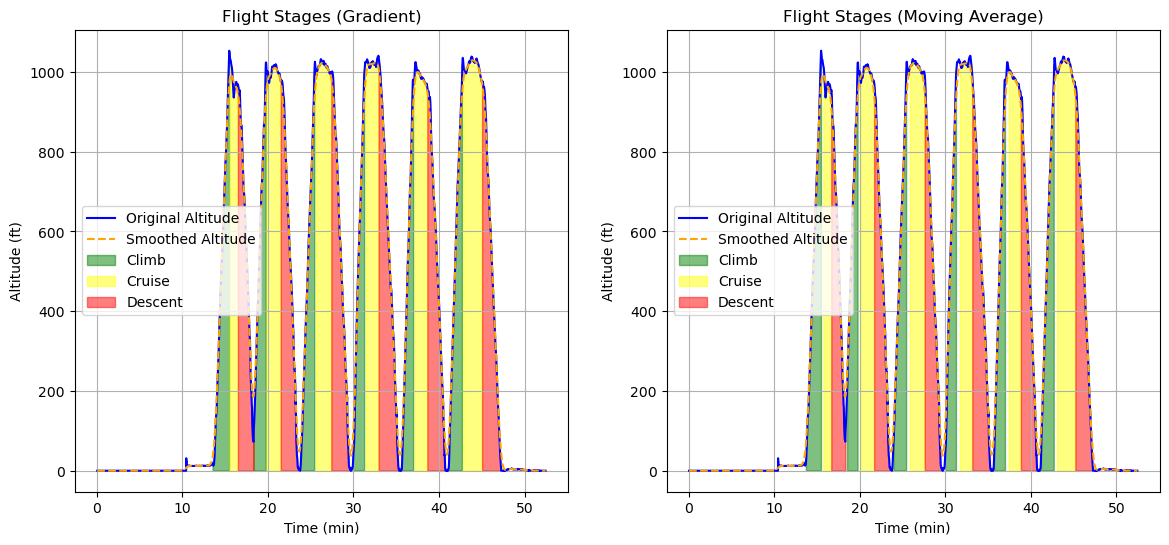
\includegraphics[width=0.95\textwidth]{flight_cell9_fig3.png}
    \caption{Representative flight-stage classification for a circuit flight at CYKF, comparing gradient-based (left) and moving-average-based (right) methods. Green indicates climb, yellow indicates cruise, and red indicates descent.}
    \label{fig:flight-stages}
\end{figure}

Analysis of battery SoC patterns across classified flight phases revealed that the climb phase accounts for the largest share of SoC depletion (Table~\ref{tab:soc-by-phase}), consistent with the high power demands during takeoff.

\begin{table}[H]
    \centering
    \caption{Average battery SoC change ($\Delta$SoC) by flight phase.}
    \label{tab:soc-by-phase}
    \begin{tabular}{lc}
        \toprule
        \textbf{Flight Phase} & \textbf{$\Delta$SoC (\%)} \\
        \midrule
        Taxi & 0.4 \\
        Climb & 6.0 \\
        Cruise & 3.7 \\
        Descent & 0.7 \\
        \bottomrule
    \end{tabular}
\end{table}

\subsection{All-Flights Altitude Overview}

Figure~\ref{fig:all-flights-alt} presents an overlay of altitude profiles for all valid circuit flights in the dataset.
The characteristic circuit pattern is clearly visible: a climb phase to approximately 1000--1200~ft, a level cruise segment, and a descent back to ground level, repeated multiple times per flight session.

\begin{figure}[H]
    \centering
    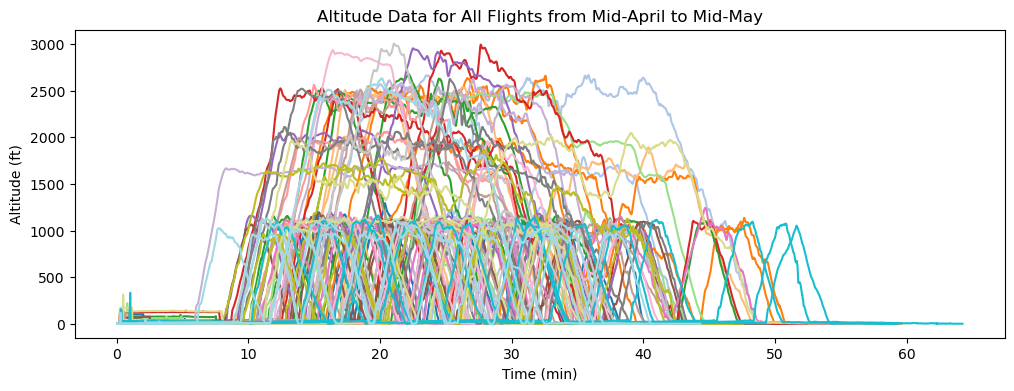
\includegraphics[width=0.85\textwidth]{outdated_cell9_fig1.png}
    \caption{Altitude versus time overlay for all valid circuit flights, color-coded by flight index. The consistent circuit pattern with maximum altitudes below 1300~ft AGL is evident.}
    \label{fig:all-flights-alt}
\end{figure}

\subsection{Energy Consumption by Flight Stage}

\subsubsection{Takeoff (Climb)}

Energy consumption during takeoff varies with the altitude band analyzed.
Table~\ref{tab:takeoff-energy} summarizes the average energy consumption and power settings for each altitude band.

\begin{table}[H]
    \centering
    \caption{Average energy consumption and power settings by altitude band during takeoff.}
    \label{tab:takeoff-energy}
    \begin{tabular}{lccc}
        \toprule
        \textbf{Altitude Band} & \textbf{Avg Power (kW)} & \textbf{Avg Energy (kWh)} & \textbf{$\Delta$SoC at 75\% SoH} \\
        \midrule
        0--300~ft (Initial) & 54.5 & 0.417 & --- \\
        300--600~ft (1st Climb) & 48.4 & 0.374 & --- \\
        600--900~ft (2nd Climb) & 47.6 & 0.368 & --- \\
        \midrule
        \textbf{Total (0--900~ft)} & --- & \textbf{1.169} & \textbf{6.285\%} \\
        \bottomrule
    \end{tabular}
\end{table}

For the initial climb (0--300~ft), where full power is typically applied, scatter plots of energy versus average power (Figure~\ref{fig:takeoff-scatter}) reveal a positive correlation between power and total energy, with data points color-coded by headwind.
The box plot analysis of energy binned by 5~kW power increments provides a statistical summary of the within-bin distribution at each power level.

\begin{figure}[H]
    \centering
    \begin{subfigure}[b]{0.58\textwidth}
        \centering
        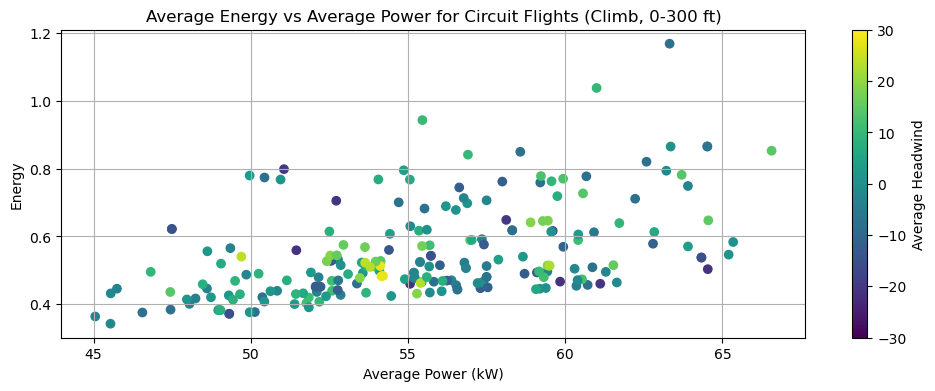
\includegraphics[width=\textwidth]{flight_cell18_fig2.png}
        \caption{Scatter plot color-coded by average headwind.}
    \end{subfigure}
    \hfill
    \begin{subfigure}[b]{0.38\textwidth}
        \centering
        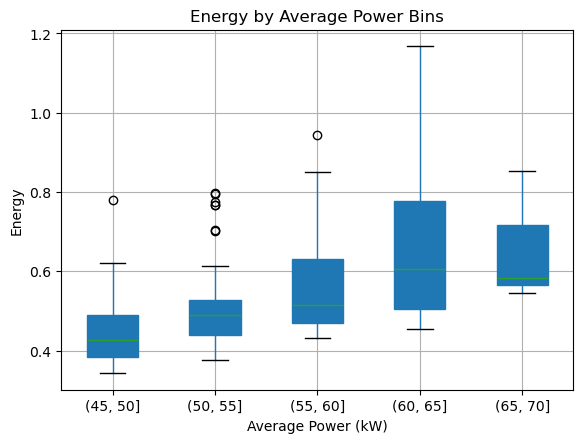
\includegraphics[width=\textwidth]{flight_cell18_fig4.png}
        \caption{Box plot by 5~kW power bins.}
    \end{subfigure}
    \caption{Energy consumption during the initial takeoff climb (0--300~ft) as a function of average motor power.}
    \label{fig:takeoff-scatter}
\end{figure}

Flights into a strong headwind exhibit elevated energy per kilometer due to reduced ground speed, while tailwind flights show reduced apparent consumption.
The adjusted energy per kilometer metric partially normalizes this effect.

Figures~\ref{fig:takeoff-full-energy} and~\ref{fig:takeoff-full-ekm} show the same analysis applied to the full takeoff phase (0--1300~ft), using total energy and energy per kilometer as the respective metrics.

\begin{figure}[H]
    \centering
    \begin{subfigure}[b]{0.58\textwidth}
        \centering
        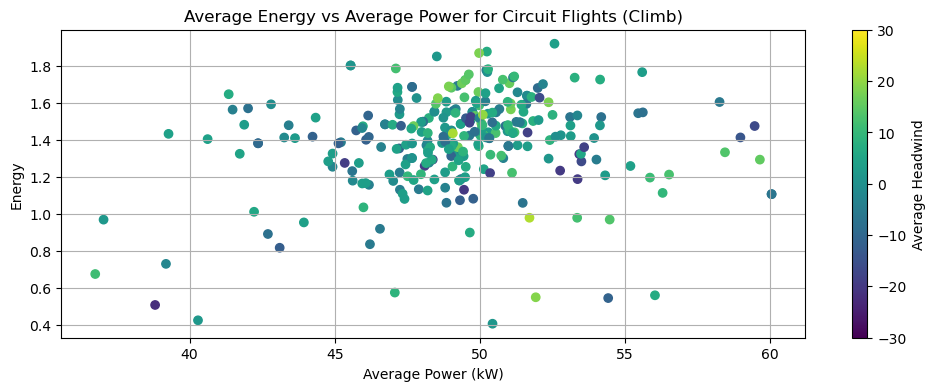
\includegraphics[width=\textwidth]{flight_cell22_fig2.png}
        \caption{Scatter plot of total energy vs.\ average power.}
    \end{subfigure}
    \hfill
    \begin{subfigure}[b]{0.38\textwidth}
        \centering
        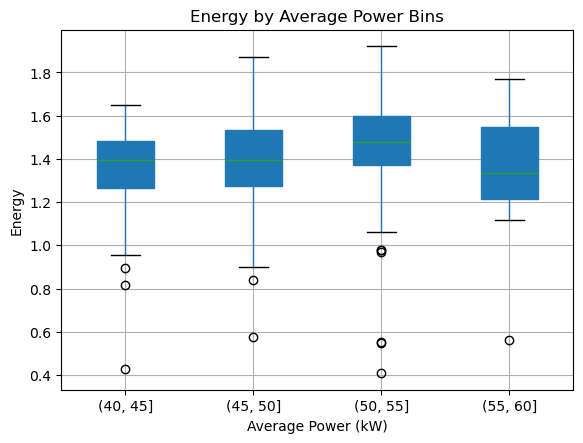
\includegraphics[width=\textwidth]{flight_cell22_fig4.png}
        \caption{Box plot by 5~kW power bins.}
    \end{subfigure}
    \caption{Total energy consumption during the full takeoff phase (0--1300~ft).}
    \label{fig:takeoff-full-energy}
\end{figure}

\begin{figure}[H]
    \centering
    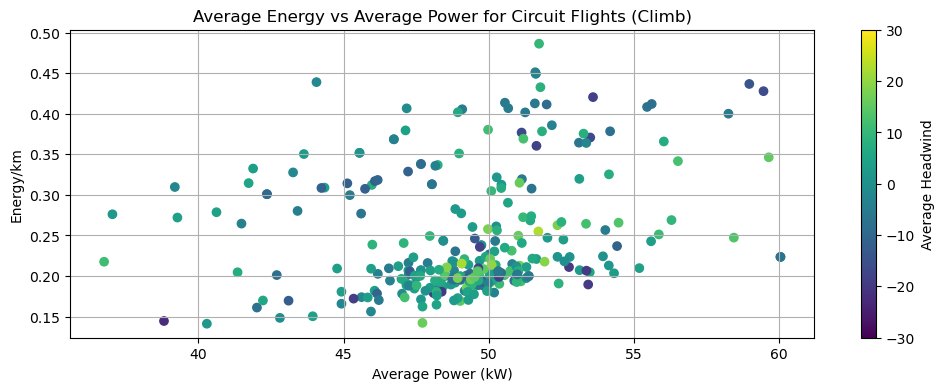
\includegraphics[width=0.6\textwidth]{flight_cell23_fig2.png}
    \caption{Energy per kilometer during the full takeoff phase, color-coded by average headwind.}
    \label{fig:takeoff-full-ekm}
\end{figure}

\subsubsection{Cruise}

Cruise energy per kilometer, measured using the adjusted (wind-corrected) metric, shows a narrower range of variability compared to the takeoff phase.
Average power during cruise typically ranges from 10 to 30~kW.
Figure~\ref{fig:cruise-energy} presents the adjusted energy per kilometer versus average power for the cruise phase.

\begin{figure}[H]
    \centering
    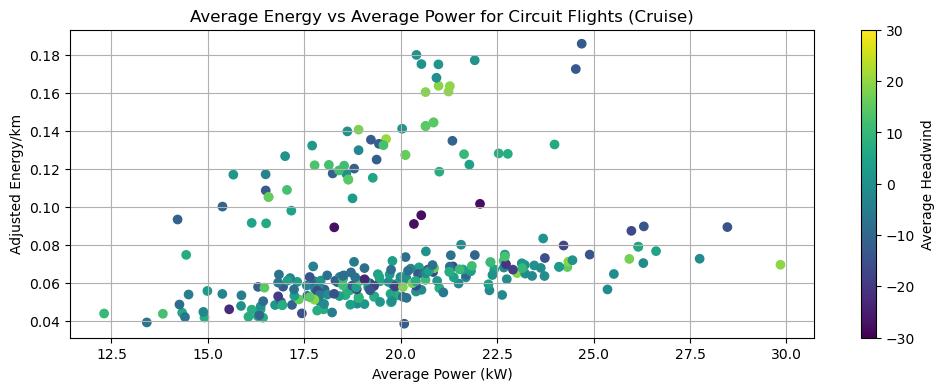
\includegraphics[width=0.6\textwidth]{flight_cell24_fig2.png}
    \caption{Adjusted energy per kilometer during the cruise phase, color-coded by average headwind.}
    \label{fig:cruise-energy}
\end{figure}

The relatively flat relationship between power setting and energy consumption per unit distance in the cruise phase suggests that the aircraft operates near its aerodynamic efficiency peak at typical circuit altitudes and speeds.

\subsubsection{Landing (Descent)}

Landing segments are dominated by low-power or idle glide configurations, with average power typically below 10~kW.
Figure~\ref{fig:landing-energy} shows the energy per kilometer versus average power for landing, which serves primarily as a baseline comparison for the energy-intensive takeoff phase.

\begin{figure}[H]
    \centering
    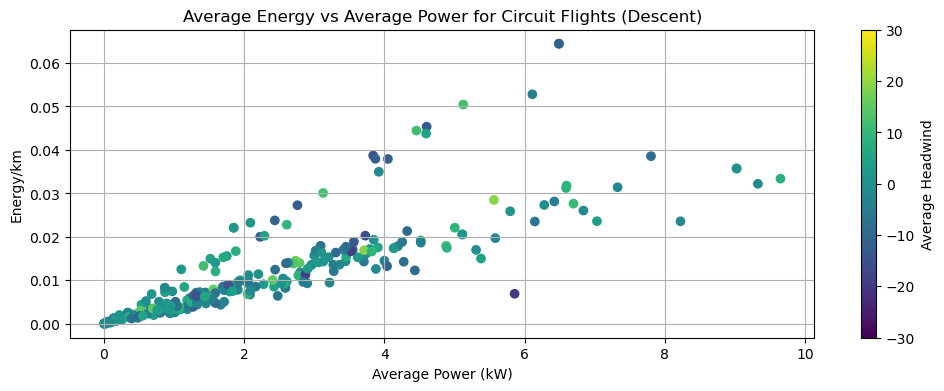
\includegraphics[width=0.6\textwidth]{flight_cell25_fig2.png}
    \caption{Energy per kilometer during the descent/landing phase.}
    \label{fig:landing-energy}
\end{figure}

\subsection{Battery State-of-Health Degradation}

Battery SoH was tracked across successive flights over the data collection period (mid-April through mid-November 2024).
Figure~\ref{fig:soh} shows the SoH trend for both Battery~1 and Battery~2.
A gradual decline is observed, consistent with expected lithium-ion aging under cyclic charge--discharge conditions typical of circuit training operations.

\begin{figure}[H]
    \centering
    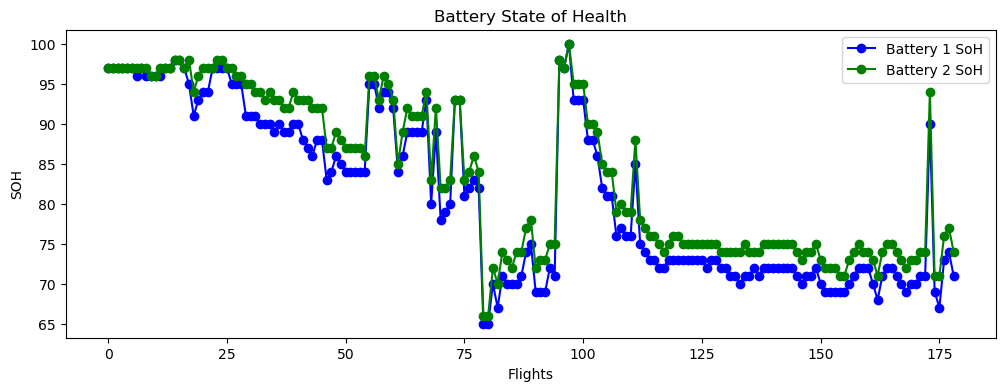
\includegraphics[width=0.7\textwidth]{outdated_cell7_fig1.png}
    \caption{Battery~1 and Battery~2 State-of-Health (SoH) plotted against successive flight indices over the observation window.}
    \label{fig:soh}
\end{figure}

Regression analysis of SoH's effect on energy consumption revealed that flights with SoH in the 70--80\% range consumed approximately 0.1~kWh more energy than those in the 80--100\% range when measured over the full takeoff to 900~ft.
At the initial takeoff stage (0--175~ft), the effect was reversed: lower SoH values were associated with marginally more efficient performance at higher power settings, though this relationship exhibited greater variance and lower statistical confidence.

\subsection{Temperature Effects}

Takeoff power data were segmented by OAT into four temperature bins ($<$15$^\circ$C, 15--17.5$^\circ$C, 17.5--20$^\circ$C, $>$20$^\circ$C).
Figure~\ref{fig:oat-power} presents a 2$\times$2 subplot of power profiles for each temperature range during the takeoff phase.

\begin{figure}[H]
    \centering
    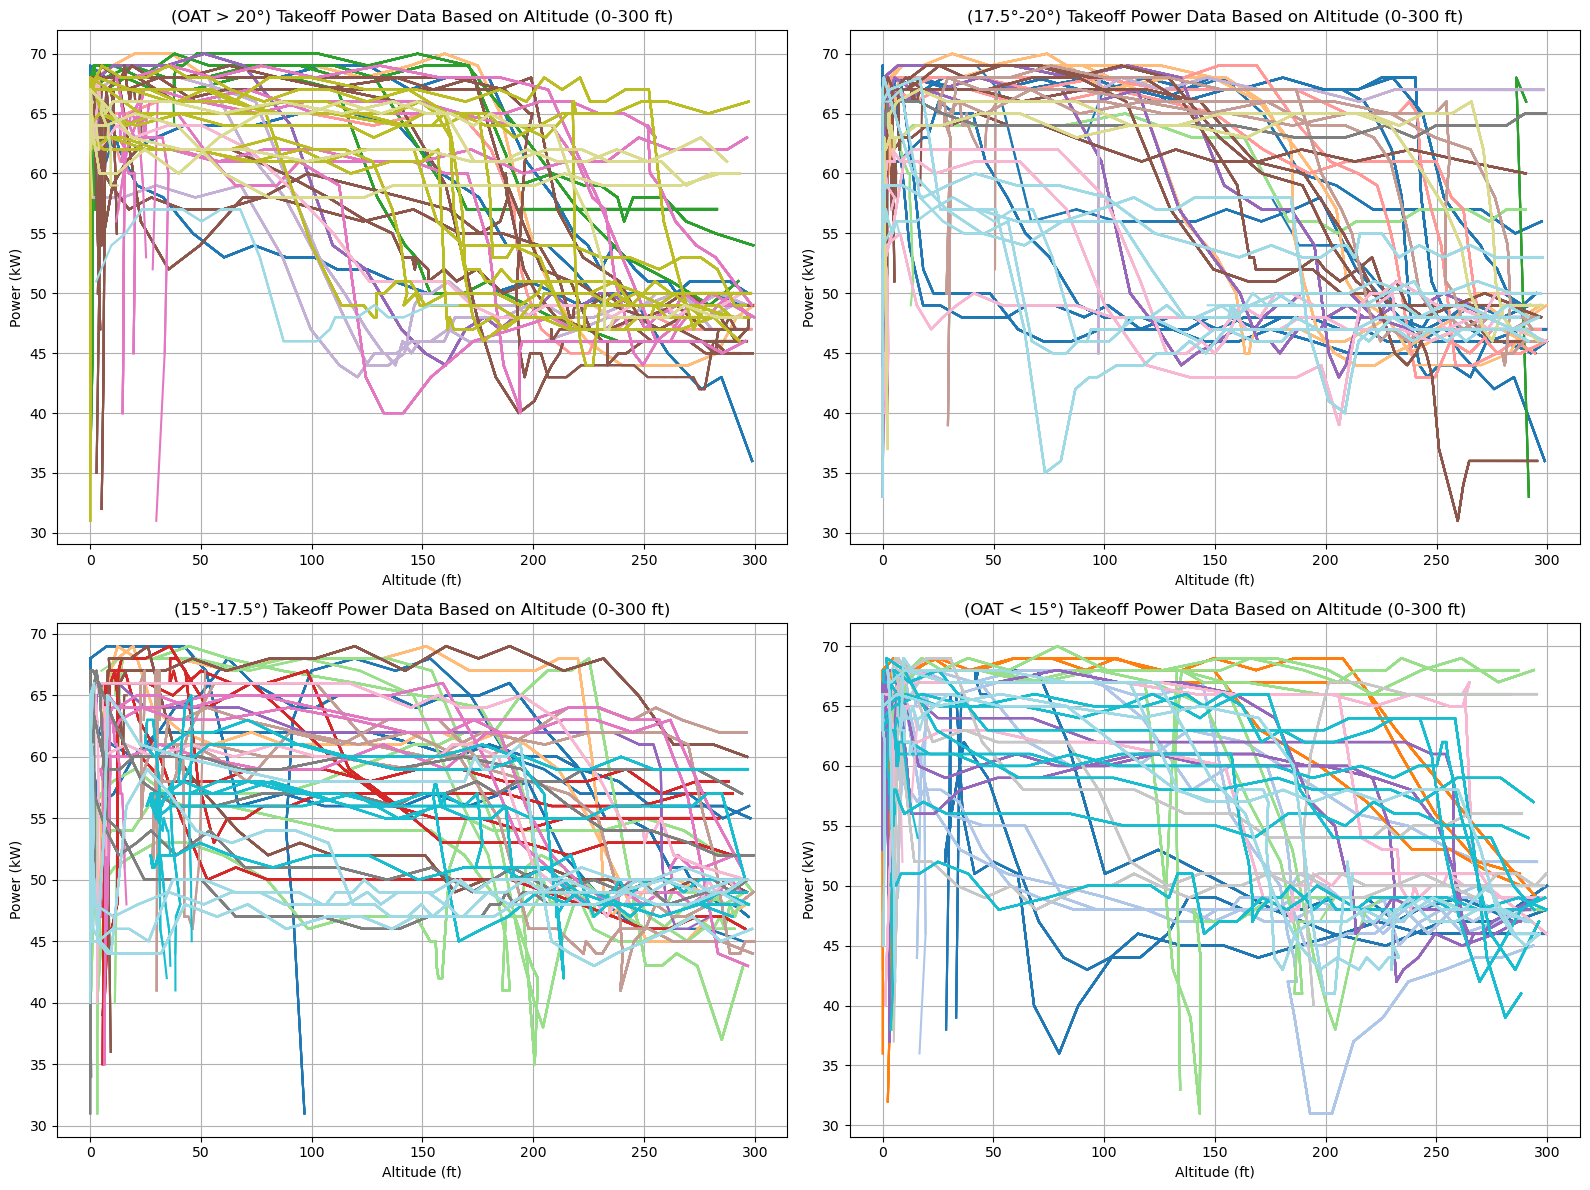
\includegraphics[width=0.85\textwidth]{outdated_cell26_fig2.png}
    \caption{Takeoff power profiles segmented by outside air temperature bins.}
    \label{fig:oat-power}
\end{figure}

For standing takeoffs, moderate correlation was observed between OAT and climb performance: the 20--25$^\circ$C range yielded the best performance at low altitudes (0--175~ft), while 5--10$^\circ$C exhibited the worst.
Higher temperatures improved initial takeoff performance---likely due to better battery electrochemical response and reduced air density---but reduced efficiency over the full 0--900~ft climb.
Rolling takeoffs showed little to no impact from varying outside temperatures, suggesting that the momentum advantages of a rolling start may dominate over temperature-driven aerodynamic differences.

Battery cell temperature also showed influence, with the 23--28$^\circ$C range performing worst at 0--175~ft (a moderately weak correlation), though these differences were deemed negligible for operational decision-making.

\subsection{Standing versus Rolling Takeoff}

The comparison between standing and rolling takeoff procedures revealed notable differences in both climb rate and energy consumption (Table~\ref{tab:standing-rolling}).

\begin{table}[H]
    \centering
    \caption{Comparison of standing vs.\ rolling takeoff performance characteristics.}
    \label{tab:standing-rolling}
    \begin{tabular}{lcc}
        \toprule
        \textbf{Metric} & \textbf{Standing} & \textbf{Rolling} \\
        \midrule
        Climb rate--power correlation & Weaker (linear) & Stronger (exponential) \\
        Speed advantage per kW & Baseline & +0.003769 min/kW faster \\
        Energy slope (0--175~ft) & $-0.0036$~kWh/kW & $-0.0056$~kWh/kW \\
        Energy slope (0--900~ft) & $-0.008956$~kWh/kW & $-0.008970$~kWh/kW \\
        45 vs 65~kW $\Delta E$ (0--175~ft) & 0.072~kWh & 0.112~kWh \\
        45 vs 65~kW $\Delta E$ (0--900~ft) & 0.18~kWh & 0.18~kWh \\
        45 vs 65~kW $\Delta$SoC (100\% SoH) & 0.75\% & 0.75\% \\
        45 vs 65~kW $\Delta$SoC (80\% SoH) & 0.94\% & 0.94\% \\
        \bottomrule
    \end{tabular}
\end{table}

Climb rate was significantly affected by power setting in both scenarios, with rolling climbs showing a more pronounced impact (strong linear and exponential increase with power) compared to standing climbs (weaker linear increase).
Rolling takeoffs consumed higher total energy at 0--175~ft when transitioning from 45 to 65~kW, but both procedures converged to nearly identical energy consumption over the full 0--900~ft climb.
The energy slopes of approximately $-0.009$~kWh/kW at 900~ft indicate that each additional kilowatt of average power reduces total takeoff energy by about 9~Wh, translating to a roughly 0.2\% decrease in SoC per 5~kW increase in average power.

\subsection{September--November Battery Profiles}

Supplementary analysis of September through November flights produced comprehensive battery discharge and power draw profiles.
Figure~\ref{fig:sep-nov} presents the four-panel overview showing SoC discharge and power for both batteries across all flights in this period.

\begin{figure}[H]
    \centering
    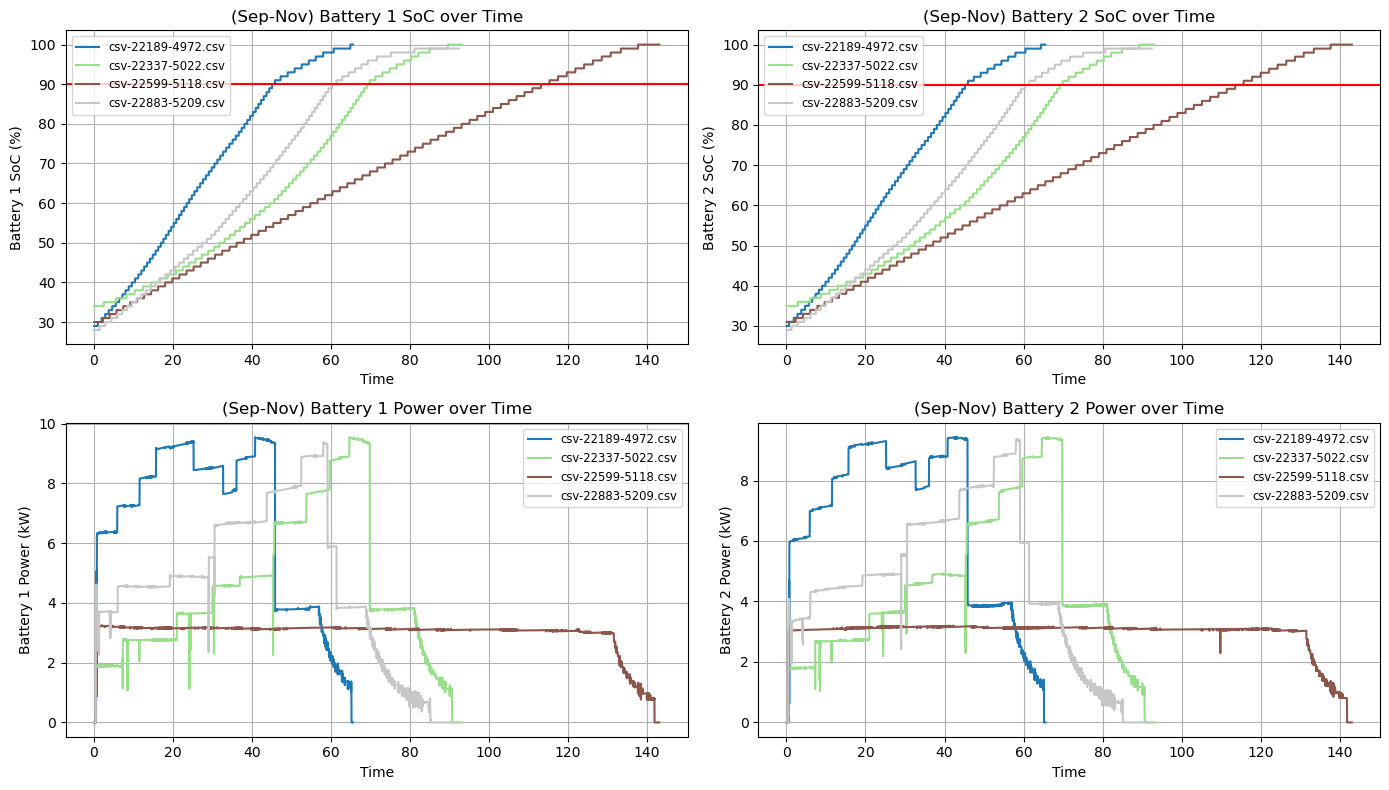
\includegraphics[width=0.85\textwidth]{misc_cell5_fig2.png}
    \caption{Battery discharge (SoC) and power profiles for September through November flights. Top: Battery~1 and Battery~2 SoC with 90\% reference line. Bottom: Battery~1 and Battery~2 power draw. Each color represents a different flight.}
    \label{fig:sep-nov}
\end{figure}

The SoC profiles exhibit characteristic sawtooth patterns corresponding to successive circuit segments, with the 90\% SoC reference line indicating flights that began below full charge.
Power profiles show the expected pattern of high-power spikes (takeoff) followed by sustained lower power (cruise) and minimal power (descent).

\subsection{Feature Importance}

Random Forest-based feature importance analysis reveals that \textbf{average power} is consistently the most influential predictor of energy consumption per kilometer across all three flight stages.
Figure~\ref{fig:feature-importance} presents the feature importance bar charts for each stage.

\begin{figure}[H]
    \centering
    \begin{subfigure}[b]{0.32\textwidth}
        \centering
        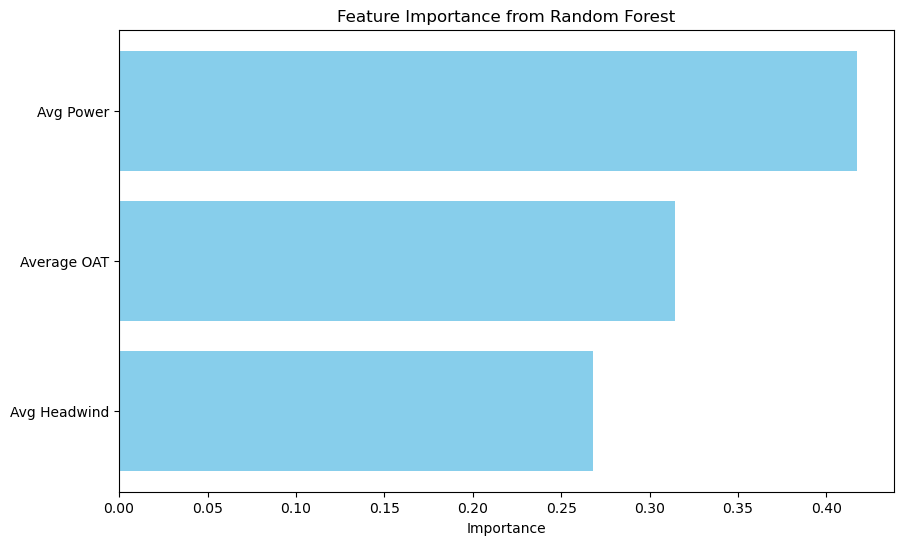
\includegraphics[width=\textwidth]{flight_cell37_fig3.png}
        \caption{Takeoff}
    \end{subfigure}
    \hfill
    \begin{subfigure}[b]{0.32\textwidth}
        \centering
        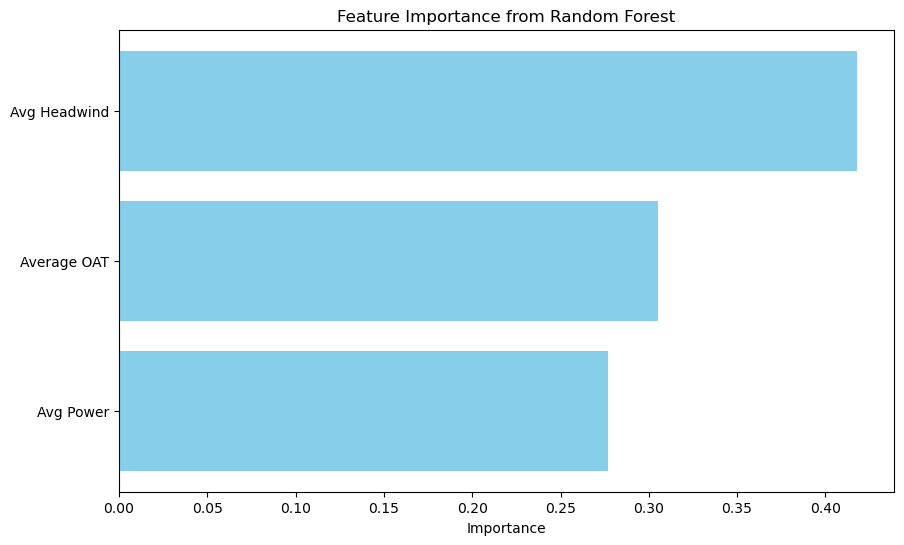
\includegraphics[width=\textwidth]{flight_cell38_fig3.png}
        \caption{Cruise}
    \end{subfigure}
    \hfill
    \begin{subfigure}[b]{0.32\textwidth}
        \centering
        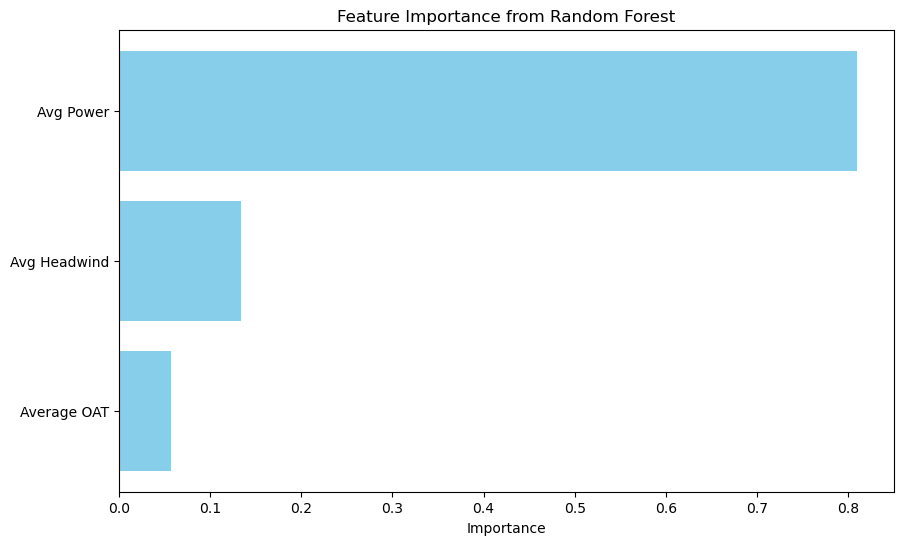
\includegraphics[width=\textwidth]{flight_cell39_fig3.png}
        \caption{Landing}
    \end{subfigure}
    \caption{Feature importance (mean decrease in impurity) from Random Forest regression for each flight stage. Features: Average Power, Average Headwind, Average OAT.}
    \label{fig:feature-importance}
\end{figure}

For the takeoff phase, average headwind ranks second, followed by average OAT.
In the cruise phase, headwind becomes relatively more important, reflecting the proportionally greater impact of wind on ground speed at lower power settings.

\subsection{XGBoost Predictive Modeling Results}

The XGBoost regressor was trained separately for each flight stage with features \{SoH, Average OAT, Avg Power, Avg Headwind\} predicting energy per kilometer.
Figure~\ref{fig:xgboost} presents the actual versus predicted scatter plots and prediction overlays for each stage.

\begin{figure}[H]
    \centering
    \begin{subfigure}[b]{0.32\textwidth}
        \centering
        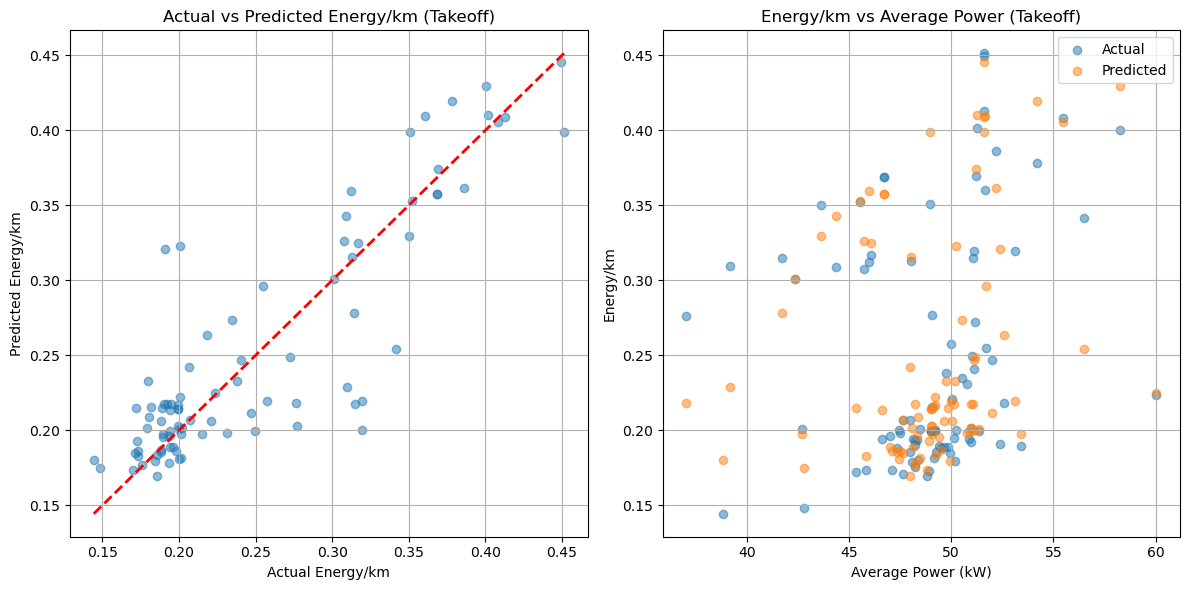
\includegraphics[width=\textwidth]{flight_cell44_fig3.png}
        \caption{Takeoff}
    \end{subfigure}
    \hfill
    \begin{subfigure}[b]{0.32\textwidth}
        \centering
        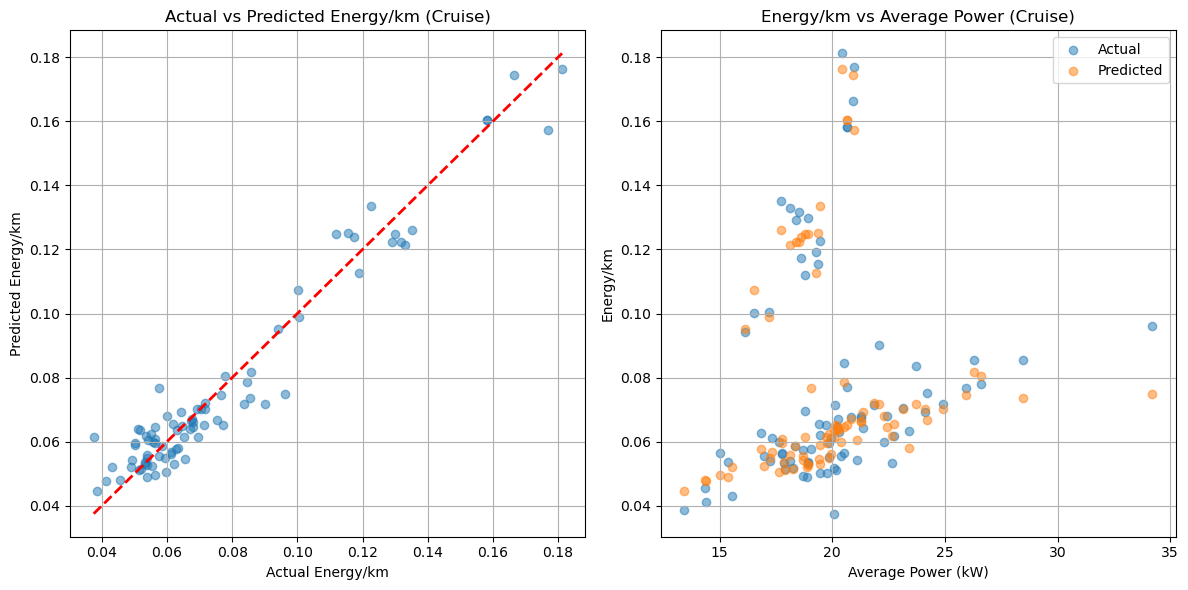
\includegraphics[width=\textwidth]{flight_cell45_fig3.png}
        \caption{Cruise}
    \end{subfigure}
    \hfill
    \begin{subfigure}[b]{0.32\textwidth}
        \centering
        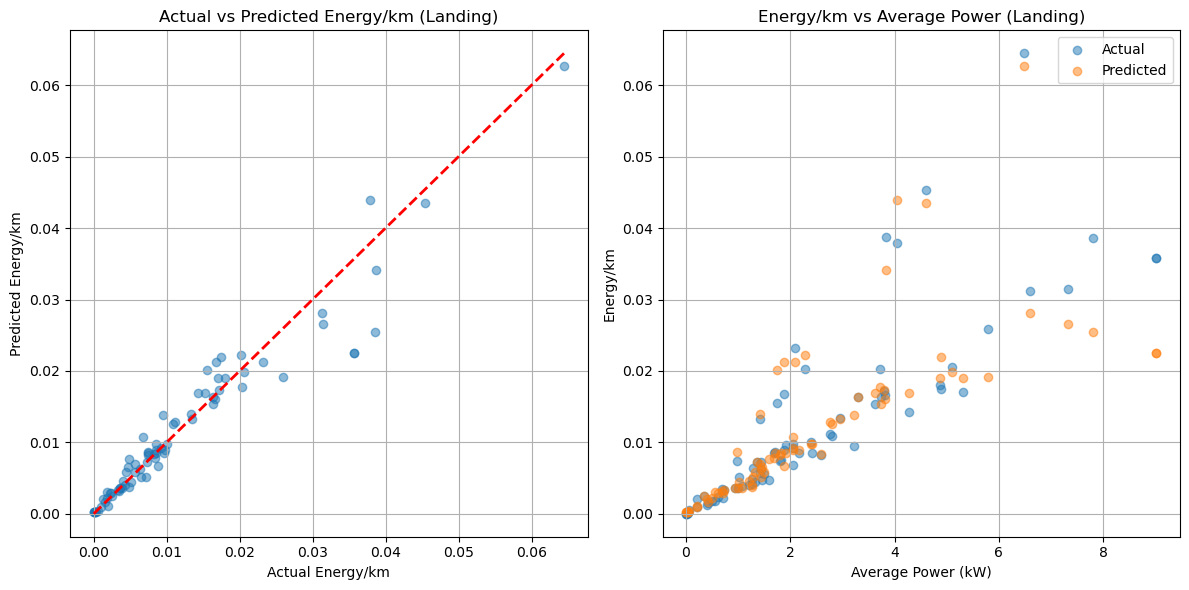
\includegraphics[width=\textwidth]{flight_cell46_fig3.png}
        \caption{Landing}
    \end{subfigure}
    \caption{XGBoost regression results for each flight stage. Left panel of each subplot: actual vs.\ predicted energy/km with identity line. Right panel: energy/km vs.\ average power with actual (blue) and predicted (orange) values overlaid.}
    \label{fig:xgboost}
\end{figure}

The cruise stage demonstrates the tightest agreement along the diagonal, reflecting the lower variability in steady-state flight.
The takeoff stage exhibits more scatter, reflecting higher variability in climb profiles and the influence of unmodeled factors such as pilot technique and aircraft weight.

\subsection{PCA Dimensionality Reduction}

Two-component PCA projections of the five-feature space provide a qualitative overview of the data structure for each flight stage (Figure~\ref{fig:pca}).
Note that standard feature scaling was not applied prior to PCA; consequently, features with larger absolute magnitudes (e.g., power in kW) disproportionately influence the principal component axes.
The resulting projections should therefore be interpreted as exploratory visualizations rather than rigorous dimensional analyses.

\begin{figure}[H]
    \centering
    \begin{subfigure}[b]{0.48\textwidth}
        \centering
        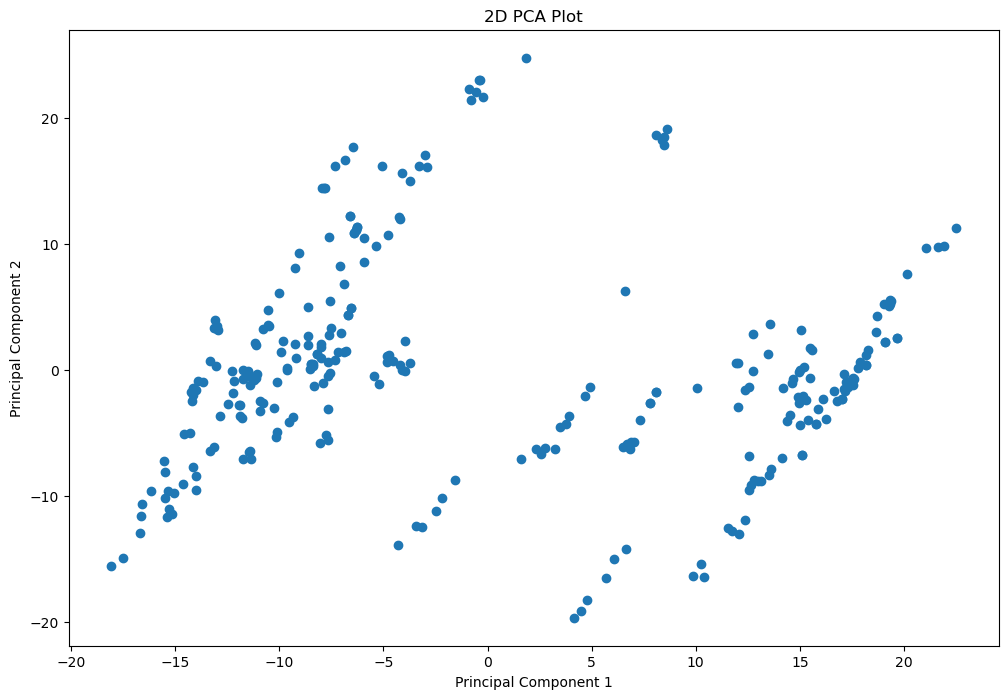
\includegraphics[width=\textwidth]{flight_cell32_fig3.png}
        \caption{Takeoff}
    \end{subfigure}
    \hfill
    \begin{subfigure}[b]{0.48\textwidth}
        \centering
        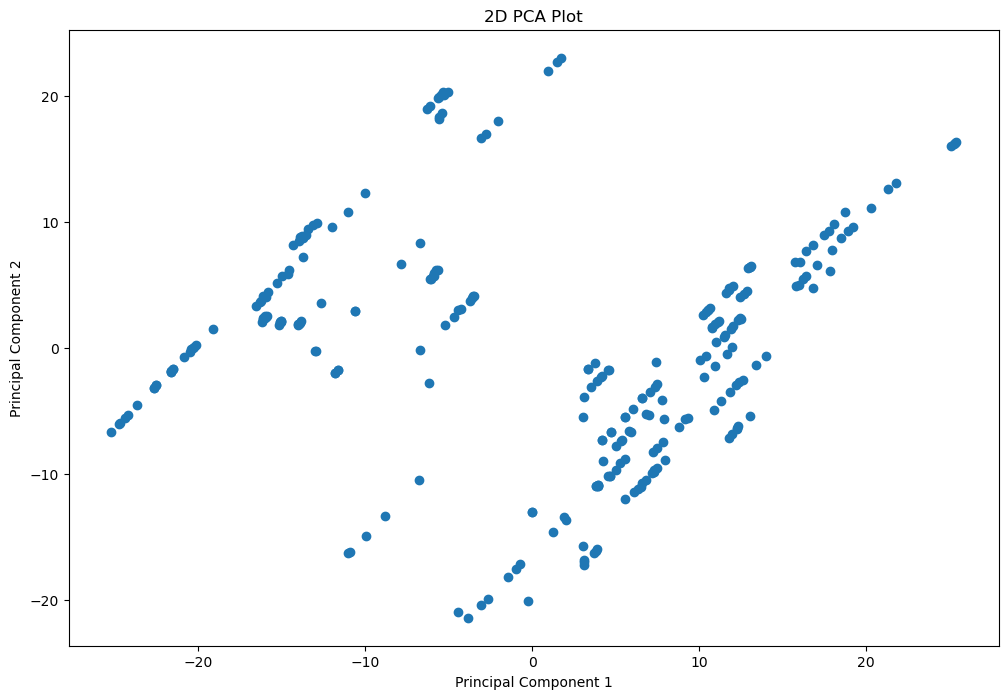
\includegraphics[width=\textwidth]{flight_cell33_fig3.png}
        \caption{Cruise}
    \end{subfigure}
    \caption{PCA projections into two principal components for the takeoff and cruise flight stages.}
    \label{fig:pca}
\end{figure}

With this caveat, the takeoff stage data forms a relatively compact cluster, consistent with the narrow operational range of power settings during climb.
The cruise stage shows more dispersion along the first principal component, likely reflecting the wider range of power and headwind conditions encountered during level flight, though the lack of feature scaling means this dispersion may partly reflect magnitude differences rather than true variance structure.

\subsection{Campbell River Comparison}

A limited comparison with flights conducted at Campbell River Airport (Vancouver Island) provided additional context.
The Campbell River data showed average takeoff energy of 1.176~kWh per takeoff (compared to 1.169~kWh at Waterloo), but with a markedly different power profile: lower initial power settings produced slightly longer takeoff durations.
The near-identical total energy consumption despite different power profiles supports the finding that total takeoff energy is relatively insensitive to the power-setting schedule within the observed range.

% ══════════════════════════════════════════════
% 6. DISCUSSION
% ══════════════════════════════════════════════
\section{Discussion}

The results of this study provide several actionable insights for the operation of the Pipistrel Velis Electro in a flight training context.

\paragraph{Power Settings and Energy Efficiency.}
Average power dominates energy consumption per kilometer across all flight stages, consistent with the fundamental relationship $E = \int P\,dt$: higher power produces faster climbs at greater energy cost per unit distance.
However, a key finding is that \emph{within the observed operational power range (approximately 45--65~kW), higher average power settings result in lower total energy consumption per takeoff}.
The negative energy slopes of approximately $-0.009$~kWh/kW at 900~ft indicate that the time savings from faster climbs outweigh the higher instantaneous power draw.
Physically, a faster climb reduces the total time spent in the high-drag, low-speed regime near the ground, and also reduces the duration over which parasitic losses (avionics, thermal management) accumulate.
This relationship is bounded: beyond the observed power range, aerodynamic drag increases nonlinearly and propulsive efficiency may decline, likely reversing the trend.
The present data do not extend to power settings above approximately 65~kW, so extrapolation beyond this regime should be avoided.

Both high and low settings within the 45--65~kW range produced similar total discharge rates, suggesting that the battery operates within its efficient electrochemical regime throughout this range.
A lower power setting, however, would be more optimal to minimize strain on the battery, theoretically reducing SoH degradation over time.

\paragraph{Wind Effects.}
Headwind was consistently identified as the second most important predictor.
The wind-adjusted energy metric provides a fairer basis for cross-flight comparison by normalizing for the substantial effect of headwind and tailwind on ground speed.
However, the hourly resolution of the ground-level wind data introduces measurement uncertainty, particularly in gusty or variable conditions.

\paragraph{Temperature.}
The OAT effect follows a nuanced pattern: higher temperatures improved performance at low altitudes (0--175~ft) through a combination of better battery electrochemical response and reduced air density, but this advantage diminished or reversed over the full climb.
Rolling takeoffs exhibited substantially less temperature sensitivity than standing takeoffs, suggesting that the aerodynamic benefits of initial momentum may buffer against atmospheric variations.

\paragraph{Standing vs.\ Rolling Takeoffs.}
Rolling climbs reach altitude 0.003769~minutes faster per kilowatt of power compared to standing climbs.
The convergence of energy consumption between standing and rolling procedures at higher altitudes (900~ft) indicates that the initial energy advantage of rolling starts is absorbed by the subsequent climb.
From an operational standpoint, either procedure is viable with minimal energy penalty, though rolling takeoffs offer marginal time and energy advantages at low altitudes.
The theoretical expectation of approximately 1\% difference between the two procedures was confirmed by the data.

\paragraph{Battery Degradation.}
SoH degradation over the six-month observation window provides preliminary evidence that circuit training operations produce gradual but measurable battery aging.
Factors that may accelerate degradation include repeated high-power discharge cycles, exposure to elevated cell temperatures during climb, and prolonged storage at high SoC between flights.
Lower SoH values (70--85\%) were associated with higher energy consumption over the full takeoff, representing a tangible operational cost of battery aging.

\paragraph{Model Performance.}
The XGBoost models demonstrate the feasibility of predicting per-circuit energy consumption from readily available operational and environmental variables.
The stronger performance on the cruise stage reflects the lower variability inherent in steady-state flight, while the weaker takeoff predictions suggest that additional features---most notably aircraft weight (see below)---would be needed to capture the full variance.
However, these results should be interpreted as a proof-of-concept rather than a production-ready predictive model.
The models were evaluated on a single 70/30 random split without $k$-fold cross-validation, confidence intervals, or error bars on performance metrics.
Future work should incorporate stratified $k$-fold cross-validation to obtain robust performance estimates, and model-agnostic interpretability methods such as SHAP (SHapley Additive exPlanations) values to provide per-feature, per-prediction attribution beyond aggregate importance rankings.

\paragraph{Aircraft Weight as Primary Confounder.}
Although aircraft weight is listed among the study limitations, it warrants explicit discussion as the most significant unmodeled variable.
Takeoff weight directly governs the energy required to gain altitude ($E \propto m g \Delta h$) and varies substantially with pilot weight, passenger presence, battery charge state, and carried equipment.
Because weight was not recorded for any flight, its variance is absorbed into the residuals of every regression model presented here.
Future integration of weight data---even approximate values---could significantly alter the observed regression slopes and improve model accuracy, particularly for the takeoff phase where the gravitational work component dominates.

% ══════════════════════════════════════════════
% 7. LIMITATIONS
% ══════════════════════════════════════════════
\section{Limitations}

Several limitations constrain the generalizability and precision of the findings:

\begin{enumerate}
    \item \textbf{Aircraft weight (primary confounder)}: The analysis does not account for aircraft weight, which varies with battery charge state, pilot and passenger weight, and carried equipment. Because gravitational work ($E = mgh$) dominates the takeoff energy budget, weight is expected to be the single largest unmodeled factor. Its absence likely inflates the residual variance in all regression models and may bias the observed power--energy slopes. Future integration of even approximate weight data could substantially alter the quantitative findings.

    \item \textbf{Single aircraft}: All data are from a single airframe, meaning that airframe-specific factors (motor degradation, propeller condition, aerodynamic state) are confounded with the environmental and operational variables under study.

    \item \textbf{Pilot variability}: Multiple pilots operated the aircraft during the data collection period, introducing uncontrolled variability in power management, climb profiles, and circuit geometry.

    \item \textbf{Wind data resolution}: Wind speed and direction are matched at hourly resolution from ground-level weather station data, which may not accurately represent conditions at circuit altitude (1000--1200~ft AGL). Humidity and condensation effects were not modeled.

    \item \textbf{PCA scaling}: The PCA implementation does not apply standard scaling prior to transformation, meaning that features with larger absolute magnitudes may disproportionately influence the principal components.

    \item \textbf{Data subsampling}: The 10$\times$ row subsampling reduces temporal resolution to approximately one reading per 10 seconds, which may miss transient power spikes or rapid altitude changes during aggressive maneuvers.

    \item \textbf{Limited SoH range}: The observed SoH range may not span a sufficient fraction of the battery's lifetime to draw robust conclusions about the long-term relationship between SoH and energy consumption.

    \item \textbf{Single aerodrome}: The majority of flights were conducted at a single airport (CYKF), limiting the generalizability of altitude-density and atmospheric findings.

    \item \textbf{Model validation}: The XGBoost models were trained and evaluated using a single 70/30 random split without cross-validation, confidence intervals, or error bars. Performance metrics (MSE, $R^2$) are therefore point estimates subject to sampling variance. $k$-fold cross-validation and SHAP-based interpretability analysis are recommended before drawing operational conclusions from the models.
\end{enumerate}

% ══════════════════════════════════════════════
% 8. FUTURE WORK
% ══════════════════════════════════════════════
\section{Future Work}

Several avenues for extending this research emerge from the current analysis:

\begin{enumerate}
    \item \textbf{Aircraft weight integration}: Incorporating takeoff weight as a feature in the predictive models would control for a major confounding variable and enable weight-specific energy optimization.

    \item \textbf{Multi-aerodrome analysis}: Aggregating data from multiple airports at different elevations and climate zones would test the generalizability of the energy models and enable density-altitude corrections.

    \item \textbf{Charging pattern analysis}: The web scraper collects charging session data, which could be analyzed to study charging efficiency, thermal behavior during charging, and the relationship between charging patterns and SoH degradation.

    \item \textbf{Humidity and atmospheric density}: Humidity and condensation effects on motor and propeller performance merit investigation, particularly for flights in varying weather conditions.

    \item \textbf{Cross-validated modeling}: Replacing the single train-test split with stratified $k$-fold cross-validation, reporting confidence intervals on MSE and $R^2$, and incorporating SHAP values for per-prediction interpretability would substantially strengthen the predictive modeling contribution.

    \item \textbf{Temporal modeling}: Incorporating time-series models (e.g., recurrent neural networks or temporal convolutional networks) that preserve the sequential nature of within-flight data could capture dynamic effects lost in circuit-averaged metrics.

    \item \textbf{Battery degradation modeling}: Developing predictive models for SoH decline based on operational history (cycle count, depth of discharge, temperature exposure) would enable proactive battery management and replacement scheduling.

    \item \textbf{Operational recommendations}: Translating the power setting optimization results into concrete pilot operating procedures (e.g., recommended power reduction altitudes) and evaluating their impact on training throughput.

    \item \textbf{Standardized PCA and clustering}: Repeating the PCA and clustering analyses with standard-scaled features would yield more interpretable principal components and enable rigorous comparison of feature contributions to variance.
\end{enumerate}

% ══════════════════════════════════════════════
% 9. PRACTICAL IMPLICATIONS
% ══════════════════════════════════════════════
\section{Practical Implications}

The findings of this study translate into several actionable recommendations for flight training operators and pilots of electric aircraft:

\begin{enumerate}
    \item \textbf{Climb power selection}: Within the 45--65~kW range, higher power settings reduce total takeoff energy by shortening the time in the high-drag, low-altitude regime. Operators may therefore prefer full-power climbs to maximize battery endurance per training session, provided the power remains within the motor's continuous rating.

    \item \textbf{Takeoff procedure}: Rolling takeoffs offer a marginal time advantage ($\approx$0.004~min/kW) and lower energy at low altitudes, but the difference is operationally negligible over the full climb. Either procedure is viable; the choice can be driven by traffic and safety considerations rather than energy optimization.

    \item \textbf{Battery management}: The observed SoH degradation of several percentage points over six months of circuit training suggests that proactive battery health monitoring should be integrated into maintenance schedules. Flights at lower SoH values consume measurably more energy per takeoff, reducing effective endurance.

    \item \textbf{Weather planning}: Headwind is the second-largest energy driver. Scheduling high-volume circuit training on calm days---or selecting runway headings that minimize headwind during the climb phase---can yield meaningful energy savings across a full training day.

    \item \textbf{Energy budgeting}: The average takeoff energy of 1.169~kWh (6.3\% $\Delta$SoC at 75\% SoH) provides a concrete planning figure. With 24.8~kWh usable capacity and appropriate reserves, operators can estimate a maximum of approximately 12--14 circuits per full charge under typical conditions, aiding sortie and scheduling decisions.
\end{enumerate}

% ══════════════════════════════════════════════
% 10. CONCLUSION
% ══════════════════════════════════════════════
\section{Conclusion}

This report has presented a comprehensive data-driven analysis of energy consumption during circuit flight training operations of the Pipistrel Velis Electro electric aircraft at the Region of Waterloo International Airport.
The research produced an end-to-end pipeline spanning automated telemetry acquisition, multi-stage data preprocessing, gradient-based flight-stage classification, wind-adjusted energy metric computation, statistical analysis, and machine learning-based predictive modeling.

Key findings include the identification of motor power as the dominant predictor of energy consumption per kilometer across all flight stages, with headwind as a significant secondary factor.
Within the observed operational range of 45--65~kW, higher average power settings produced more energy-efficient takeoffs when measured over the full climb, with negative energy slopes of approximately $-0.009$~kWh/kW translating to roughly 0.2\% SoC savings per 5~kW increase through 900~ft.
This relationship is bounded by the operational power range studied; extrapolation beyond 65~kW is not supported by the data.
Average total takeoff energy was measured at 1.169~kWh per takeoff (6.285\% $\Delta$SoC at 75\% SoH), with near-identical values observed at a geographically distinct airport, suggesting some generalizability of the finding.

The wind-adjusted energy metric provides a fairer basis for cross-flight comparison by normalizing for headwind effects.
Rolling takeoffs offer marginal time and energy advantages at low altitudes but converge with standing takeoffs over the full climb.
Battery SoH degradation was tracked over six months of operations, providing empirical data on real-world aging under circuit training loads.

The XGBoost models demonstrate the feasibility of predicting per-circuit energy consumption from operational and environmental variables, though the single train-test split evaluation means these results should be treated as a proof-of-concept pending more rigorous cross-validated assessment.
Aircraft weight remains the most significant unmodeled variable and its future integration is expected to yield the largest improvement in predictive accuracy.
The iterative evolution of the analysis pipeline highlights the importance of noise-robust signal processing and physically grounded metric design in extracting reliable insights from real-world flight telemetry.

This work contributes to the emerging field of electric aircraft operations research, providing empirical data and analytical tools that can inform flight training procedures, battery management strategies, and the development of energy-aware flight planning systems for electric aviation.

% ══════════════════════════════════════════════
% REFERENCES
% ══════════════════════════════════════════════
\newpage
\begin{thebibliography}{10}

\bibitem{pipistrel_poh}
Pipistrel Aircraft, ``Velis Electro Pilot's Operating Handbook,'' Pipistrel d.o.o., Ajdov\v{s}\v{c}ina, Slovenia, 2020.

\bibitem{pipistrel_amm}
Pipistrel Aircraft, ``Aircraft Maintenance Manual---Velis Electro,'' Pipistrel d.o.o., Ajdov\v{s}\v{c}ina, Slovenia.

\bibitem{eccc}
Environment and Climate Change Canada, ``Historical Weather Data,'' Government of Canada. Available: \url{https://climate.weather.gc.ca/}.

\bibitem{chen2016}
T.~Chen and C.~Guestrin, ``XGBoost: A Scalable Tree Boosting System,'' in \textit{Proc.\ 22nd ACM SIGKDD Int.\ Conf.\ on Knowledge Discovery and Data Mining}, pp.~785--794, 2016.

\bibitem{breiman2001}
L.~Breiman, ``Random Forests,'' \textit{Machine Learning}, vol.~45, pp.~5--32, 2001.

\bibitem{sklearn}
F.~Pedregosa \textit{et al.}, ``Scikit-learn: Machine Learning in Python,'' \textit{J.\ of Machine Learning Research}, vol.~12, pp.~2825--2830, 2011.

\bibitem{killick2012}
R.~Killick, P.~Fearnhead, and I.~A.~Eckley, ``Optimal Detection of Changepoints with a Linear Computational Cost,'' \textit{J.\ of the American Statistical Association}, vol.~107, no.~500, pp.~1590--1598, 2012.

\bibitem{easa_tc}
European Union Aviation Safety Agency (EASA), ``Type Certificate Data Sheet No.\ EASA.A.573 for Velis Electro,'' EASA, 2020.

\end{thebibliography}

\end{document}
